\part{Basics}
\frame{\partpage}

{
\section{Topics Covered}
\usebackgroundtemplate{
\includegraphics[width=\paperwidth]{footer_4}}%
\begin{frame}{Basics: Topics Covered}

\begin{multicols}{2}
\begin{itemize}
\item Hardware
\item Storage
\item Access
\item User Environment
\item Software

\columnbreak

\item Containers
\item SLURM
\item Model Ensembler
\item Best Practise
\item HELP!
\end{itemize}
\end{multicols}
\end{frame}
}

{
\section{Hardware}
\usebackgroundtemplate{
\includegraphics[width=\paperwidth]{footer_5}}%
\begin{frame}{Access: Hardware}
\begin{itemize}
\item Gateway or Bastion hosts (bslcenb & bslcenc)
\begin{itemize}
\item Only use for access to BAS or transferring files, don’t use for running programs
\end{itemize}
\item Headnodes
	\begin{itemize}
	\item No access, manages job queues and storage (/data/hpcdata)
	\end{itemize}
\item General Use Workstations & Private Workstations
\item Nodes
\item GPU Nodes
	\begin{itemize}
	\item Currently only available for use BAS AI Lab members
	\end{itemize}	
\item Development Workstation and Development Node
	\begin{itemize}
	\item  No access, used for testing by IT
	\end{itemize}
\end{itemize}
\end{frame}
}

{
\section{Access: Authentication}
\usebackgroundtemplate{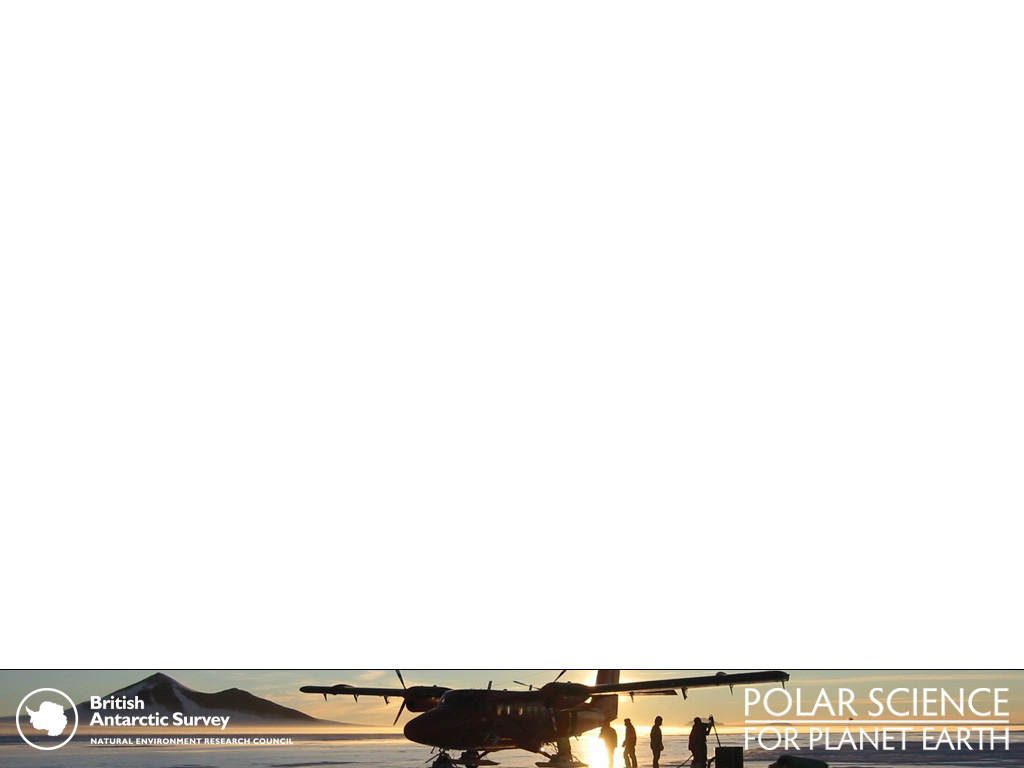
\includegraphics[width=\paperwidth]{footer_6}}%
\begin{frame}{Authentication}
\begin{itemize}
\item Three passwords – UNIX (NIS), LDAP and Samba
\item UNIX for bslcenb / bslcenc and LDAP for HPC workstations
\item Try to keep all these password synchronised
\item We are working to simplify the situation
\end{itemize}
\end{frame}
}

{
\section{Access: SSH}
\usebackgroundtemplate{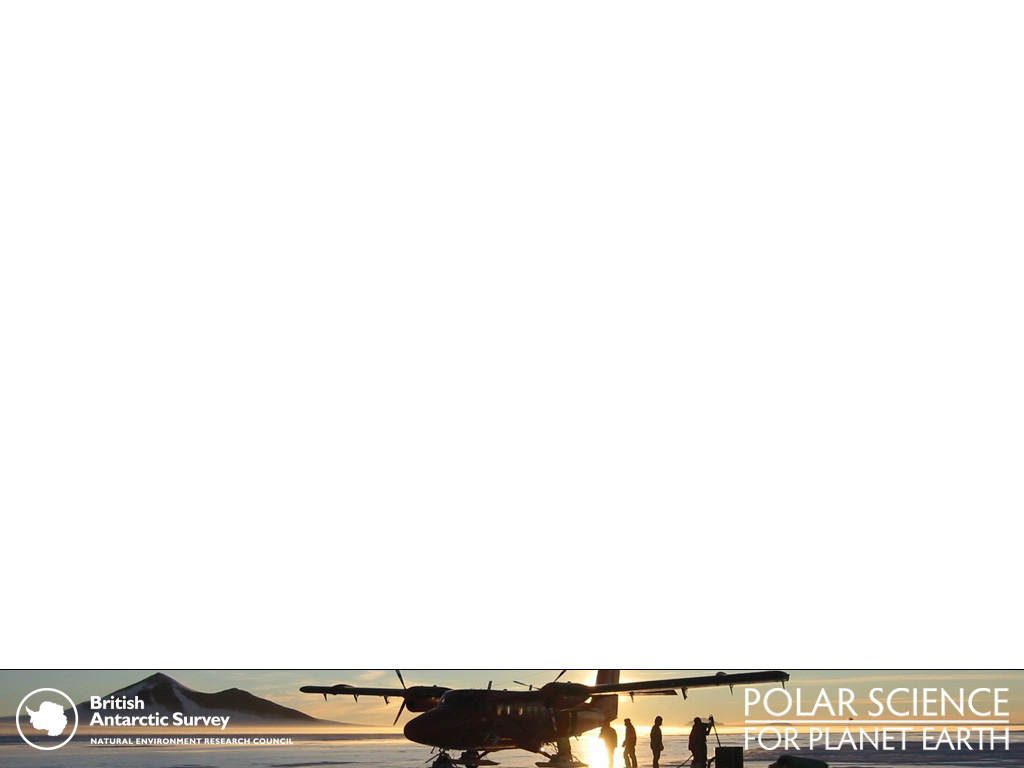
\includegraphics[width=\paperwidth]{footer_6}}%
\begin{frame}{SSH}
\begin{itemize}
\item First connect to gateway hosts: bslcenb.nerc-bas.ac.uk / bslcenc.nerc-bas.ac.uk
\item Second connect to HPC workstations: bslws01 – bslws12
\item OpenSSH (available for Linux, Mac & windows), Putty, WSL, MobaXterm
\end{itemize}
\text Demonstration
\end{frame}
}

{
\section{Access: X2go}
\usebackgroundtemplate{
\includegraphics[width=\paperwidth]{footer_8}}%
\begin{frame}{x2go}
\begin{itemize}
\item Access HPC desktop interface with or without VPN access
\item Disconnecting and reconnecting
\item Copy/paste
\item Sharing files from your laptop or PC
\item More information: \href{http://ictdocs/wiki/index.php/HPC:X2GO}{http://ictdocs/wiki/index.php/HPC:X2GO}
\pause
\item{{\color{red}Demonstration}}
\end{itemize}
\end{frame}
}

{
\section{Access: X2go alternatives}
\usebackgroundtemplate{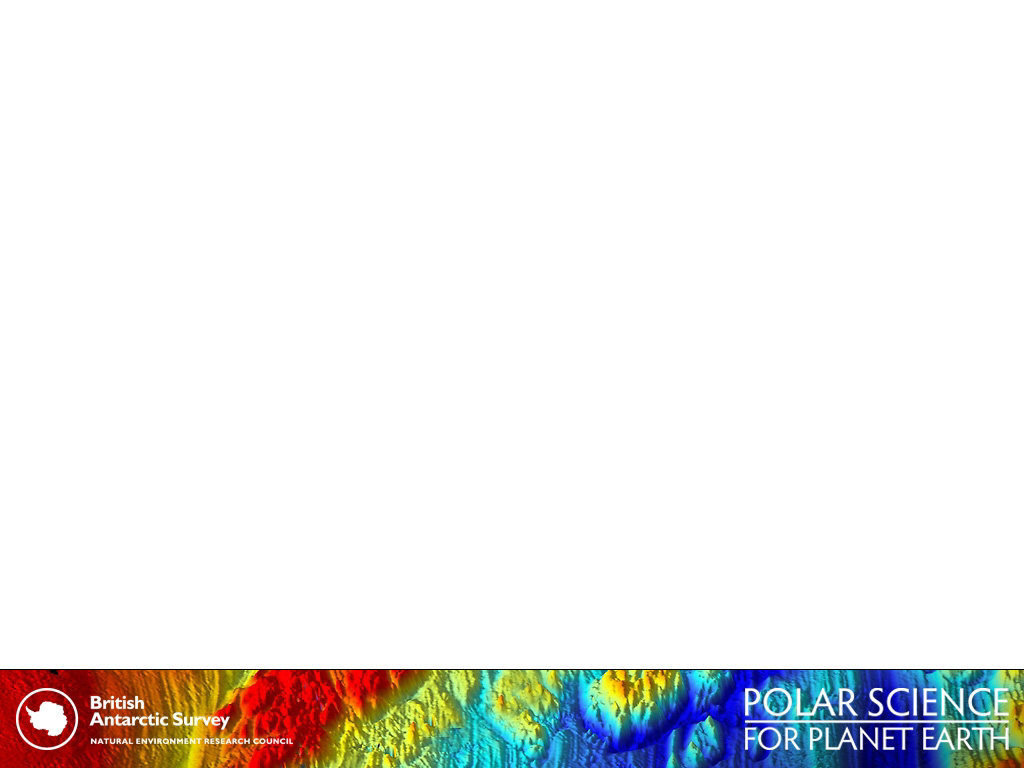
\includegraphics[width=\paperwidth]{footer_1}}%
\begin{frame}{x2go alternatives}
\begin{itemize}
\item Exceed / XMing
\item MobaXterm
\pause
\item{{\color{red}Demonstration}}
\end{itemize}
\end{frame}
}

{
\section{Access: Storage - homes}
\usebackgroundtemplate{
\includegraphics[width=\paperwidth]{footer_2}}%
\begin{frame}{Storage}
\text User Area - /users/\<username>\
\begin{itemize}
\item Small, not intended for sharing data
\item Space restricted via quotas
\item Not accessible from the HPC Nodes!
\end{itemize}
\text HPC Storage - /data/hpcdata/users/username
\begin{itemize}
\item Accessible from nodes and workstations, bslcenb, bslcenc.
\item Usage limited via quotas
\end{itemize}
\end{frame}
}

{
\section{Access: Storage SAN}
\usebackgroundtemplate{
\includegraphics[width=\paperwidth]{footer_3}}%
\begin{frame}{Storage SAN Volumes}
\begin{itemize}
\item Setup for projects and departments, eg: : /data/cruise, /data/vlf
\item Accessible from workstations, bslcenb, bslcenc
\item Volume should be managed and curated by a data manager
\item Space is not controlled by quota's
\item Adding additional space depends availability of physical disk space
\item Contact data manager first if you think you require additional storage
\end{itemize}
\end{frame}
}

{
\section{Access: Quotas}
\usebackgroundtemplate{
\includegraphics[width=\paperwidth]{footer_4}}%
\begin{frame}{Storage policies}
\text Quotas
\begin{itemize}
\item On HPC you can check your quotas using: myquota
\item Need more space - contact the service desk
\end{itemize}
\text Backups
\begin{itemize}
\item Daily at 6pm
\item All SAN and HPC volumes backed up
\item Backups are both onsite and offsite, via tapes & disk
\item If you need a file restored, contact the service desk
\end{itemize}
\end{frame}
}

{
\section{Access: Data access}
\usebackgroundtemplate{
\includegraphics[width=\paperwidth]{footer_5}}%
\begin{frame}{Data access}
\text Samba
\begin{itemize}
\item Allows clients to connect to UNIX storage as if it were a windows network share.
\item Allows access to SAN volumes, /users and /data/hpcdata
\item No access to /data/hpcflash
\end{itemize}
\end{frame}
}

{
\section{Access: SFTP}
\usebackgroundtemplate{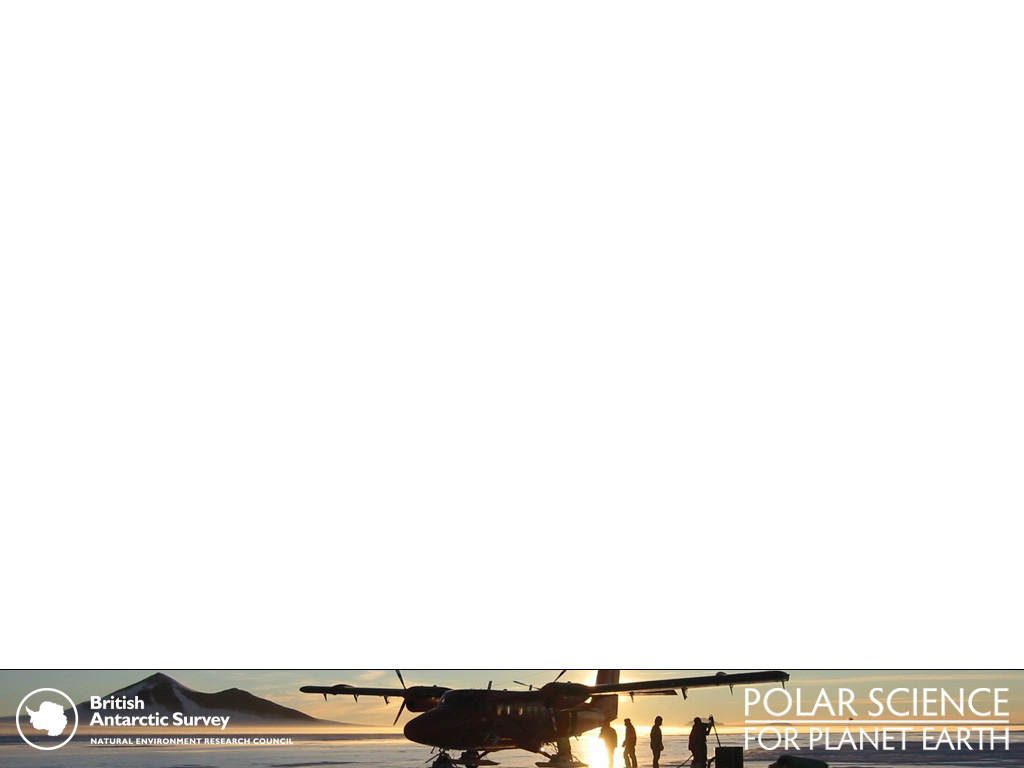
\includegraphics[width=\paperwidth]{footer_6}}%
\begin{frame}{SFTP}
\text SFTP
\begin{itemize}
\item Allows non-BAS users to retrieve files from the FTP area \href{ftp://ftp.bas.ac.uk/}{ftp://ftp.bas.ac.uk/}
\item  Users within BAS can gain access to this area and deposit files
\item Please contact the IT ServiceDesk to have a directory setup ie. /data/ftp/username
\end{itemize}
\text Writeable FTP Area
\begin{itemize}
\item Possible for non-BAS users to upload files as well, please contact the IT ServiceDesk for details
\end{itemize}
\end{frame}
}

{
\section{Access: Data access (continued)}
\usebackgroundtemplate{
\includegraphics[width=\paperwidth]{footer_7}}%
\begin{frame}{Data access (continued)}
\text rsync
\begin{itemize}
\item Perfect tool for transferring file locally and securely over the internet
\item Options to resume, reconnect, compression, limit transferred rates.
\end{itemize}
\text scp
\text sshfs
\end{frame}
}

